\subsection{Einführung} % (fold)
\label{sub:Einführung}
\begin{frame}
    \frametitle{Einführung}
    \framesubtitle{}
    \begin{block}{Versuchsziel}     
        \begin{itemize}
            \item Untersuchen des Verhaltens verschiedener Messwiderstände
        \end{itemize}
    \end{block}
    \begin{columns}[c]
        \column{0.2\textwidth}
            \begin{figure}[H]
            \begin{center}
                    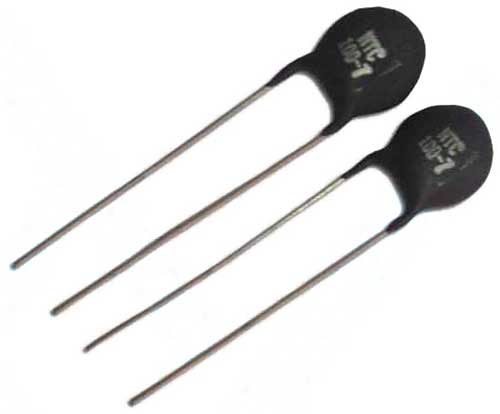
\includegraphics[scale=0.1]{./img/misc/thermistor.jpg}
            \end{center}
            \end{figure}
        \column{0.2\textwidth}
            \begin{figure}[H]
            \begin{center}
                    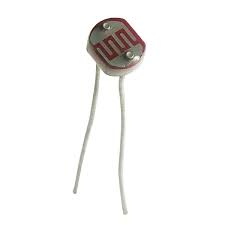
\includegraphics[scale=0.1]{./img/misc/ldr.jpeg}
            \end{center}
            \end{figure}
        \column{0.2\textwidth}
            \begin{figure}[H]
            \begin{center}
                    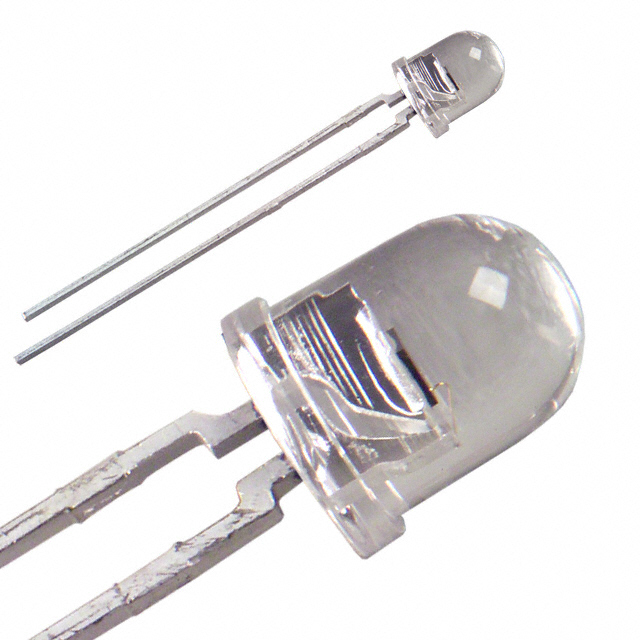
\includegraphics[scale=0.1]{./img/misc/photodiode.jpg}
            \end{center}
            \end{figure}
        \column{0.2\textwidth}
            \begin{figure}[H]
            \begin{center}
                    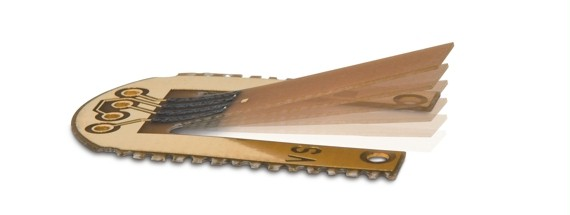
\includegraphics[scale=0.1]{./img/misc/kraftsensor.jpg}
            \end{center}
            \end{figure}
    \end{columns}
\end{frame}
% subsection Einführung (end)
